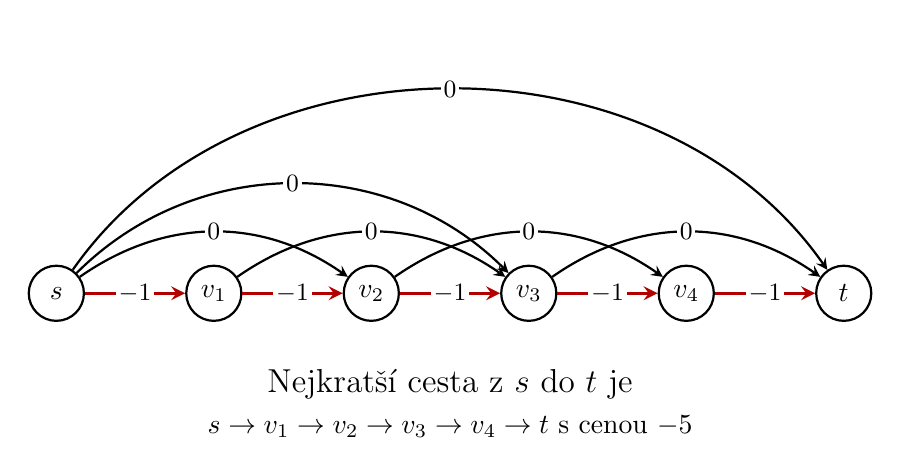
\begin{tikzpicture}[
    scale=1,
    vertex/.style={draw, circle, thick, minimum size=7mm, inner sep=0pt},
    diredge/.style={->, thick, >=stealth},
    bestedge/.style={->, very thick, draw=red!70!black, >=stealth},
    weight/.style={fill=white, inner sep=1pt, font=\small}
]

\node[vertex] (s)  at (0,0) {$s$};
\node[vertex] (v1) at (2,0) {$v_1$};
\node[vertex] (v2) at (4,0) {$v_2$};
\node[vertex] (v3) at (6,0) {$v_3$};
\node[vertex] (v4) at (8,0) {$v_4$};
\node[vertex] (t)  at (10,0) {$t$};

% Hamiltonovská cesta
\draw[bestedge] (s)  -- node[weight] {$-1$} (v1);
\draw[bestedge] (v1) -- node[weight] {$-1$} (v2);
\draw[bestedge] (v2) -- node[weight] {$-1$} (v3);
\draw[bestedge] (v3) -- node[weight] {$-1$} (v4);
\draw[bestedge] (v4) -- node[weight] {$-1$} (t);

% "kratší" lokální alternativy, které ale nejsou globálně nejlepší
\draw[diredge] (s) to[bend left=35] node[weight] {$0$} (v2);
\draw[diredge] (s) to[bend left=45] node[weight] {$0$} (v3);
\draw[diredge] (s) to[bend left=55] node[weight] {$0$} (t);

\draw[diredge] (v1) to[bend left=35] node[weight] {$0$} (v3);
\draw[diredge] (v2) to[bend left=35] node[weight] {$0$} (v4);
\draw[diredge] (v3) to[bend left=35] node[weight] {$0$} (t);

\node[align=center] at (5,-1.4)
{\large Nejkratší cesta z~$s$ do~$t$ je\\[1mm]
$s\to v_1\to v_2\to v_3\to v_4\to t$ s~cenou $-5$};

\end{tikzpicture}